\documentclass[12pt,a4paper]{scrartcl}
\usepackage[utf8]{inputenc}
\usepackage{csquotes}
\usepackage[ngerman]{babel}
\usepackage{amsmath}
\usepackage{amsfonts}
\usepackage{amssymb}
\usepackage{graphicx}
\usepackage{gensymb}
\usepackage{float}
\usepackage{microtype}
\usepackage[per-mode = fraction]{siunitx}
\usepackage[backend=biber]{biblatex}
\addbibresource{./sources.bib}
\author{Leon Bentrup}
\title{GPS}
\subtitle{Satellitennavigation}
\begin{document}
\maketitle
\tableofcontents
\newpage
\KOMAoptions{parskip=full}

\section{Vorwort}
\section{Navigation}
Die Satellitengestützten Navigationssysteme, die wir heute Verwenden, verwenden das gleiche Grundlegende Prinzip, das auch schon die Seefahrer der antike eingesetzt haben, wenn sie sich an den Sternen orientiert haben.

Man verwendet Objekte im Weltall, deren Position man kennt, um die eigene Position auf der Erde zu bestimmen.

\subsection{Sextant}
Mit einem Sextanten bestimmt man den eigenen Breitengrad mit Hilfe von drei Sternen.
Zuerst muss der Höhenwinkel von drei bekannten Sternen gemessen werden. Der Höhenwinkel ist der Winkel zwischen Horizont, dem Betrachter und dem Stern.
Danach entnimmt man aus einem Nautischen Almanach die Koordinaten der angepeilten Sterne. Aus diesen drei Messungen ergeben sich dann drei Kegel. Sie sind durch den Stern als Spitze und durch den gemessenen Höhenwinkel als Winkel zwischen Boden und Mantelfläche des Kegels genau definiert. Die Kanten zwischen Boden und Mantel schneiden sich in einem Punkt. Dieser Schnittpunkt ist die eigene Position.

\begin{figure}[H]
\centering
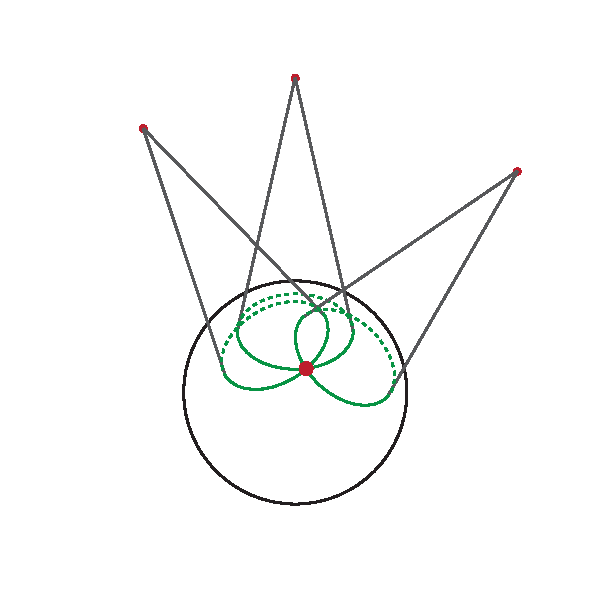
\includegraphics[width=0.7\textwidth]{img/earth_cones.pdf}
\caption{Positionsbestimmung anhand der Höhenwinkel von drei Sternen}
\end{figure}

\subsection{Koordinatensystem der Erde}
Um eine Position auf der Erde anzugeben verwendet man kein „normales“ Koordinatensystem, mit X-, Y- und Z-Koordinaten. Denn da die Erden eine Kugel (Ellipsoid) ist, und die Oberfläche gekrümmt ist, kann man mit solch einem Koordinatensystem nicht einfach rechnen. Würde man die Koordinaten für zwei Punkte am Boden und an der Spitze eines Turms angeben, müsste man dafür nicht nur eine Koordinate anpassen, sondern wahrscheinlich alle 3, um vom einen Punkt auf den anderen zu kommen.

Deshalb verwendet man in der Navigation ein System von Längengraden, Breitengraden und der Höhe über dem Meeresspiegel.

\paragraph{Breitengrade} Die Breitengrade verlaufen parallel zum Äquator der Erde. Sie reichen dabei von 90\degree{} Nord (oder nur 90\degree), der Nordpol über 0\degree, der Äquator bis 90\degree{} Süd (oder -90\degree), der Südpol. Ein Breitengrad ist also der Winkel zwischen Äquator, Erdmittelpunkt und dem zugehörigen Punkt auf der Erdoberfläche.

\paragraph{Längengrade}

\paragraph{Höhe}

\section{GPS-System}

\subsection{Segmente}
Das GPS-System wird in drei Segmente eingeteilt. Diese sind:
\begin{itemize}
\item Das Space Sagment, die Satelliten im Weltall
\item Das Control Segment, mehrere weltweit verteilte Bodenstationen zur Überwachung und Steuerung der GPS-Satelliten
\item Das User Segment, die Nutzer des GPS-Systems, also die GPS-Empfänger
\end{itemize}
\cite{gpsgov_segments}

\subsection{GPS-Satellit}
Ein GPS-Satellit umkreist die Erde in einer Höhe von ca. \SI{26600}{\kilo\meter}.
Mit dem 3. keplerschen Gesetz \eqref{eq:kepler3} kann man daraus die Umlaufzeit $T$ berechnen.

\begin{equation}
\label{eq:kepler3}
T^2 = \frac{4 \pi^2}{G (M + m)} \cdot a^3
\end{equation}
\cite{wiki_kepler}

Die Masse des Satelliten ist dabei im Vergleich zur Erdmasse vernachlässigbar.

\begin{align*}
a &= \SI{26600}{\kilo\meter} && \text{Abstand des Satelliten}\\
M &= \SI{5.97219e24}{\kilo\gram} && \text{Masse der Erde}\\
G &= \SI{6.67408e-11}{\cubic\meter\per\kilo\gram\per\square\second} && \text{Gravitationskonstante} \\
T^2 &= \frac{4 \pi^2}{G M} \cdot a^3 \\
T &= \sqrt{\frac{4 \pi^2}{\SI{6.67408e-11}{\cubic\meter\per\kilo\gram\per\square\second} \cdot \SI{5.97219e24}{\kilo\gram}} \cdot (\SI{26600}{\kilo\meter})^3} \\
T &= \SI{11.9932}{\hour} && \text{11 Stunden und 58 Minuten}
\end{align*}

Die Position der GPS-Satelliten ist also von der Erde aus gesehen nicht immer gleich, sondern sie Umkreisen die Erde zwei mal pro Tag.

\subsection{Konstellation}

\section{GPS-Signal}
\begin{equation}
f_{L_1} = \SI{1.57542}{\giga\hertz} \nonumber
\end{equation}

\subsection{CDMA}

Um dennoch die Signale verschiedener Satelliten unterscheiden zu können (auch wenn sich ihre Signale überlagern, da von allen die gleiche Frequenz benutzt wird), wird eine Technik namens CDMA angewendet.
CDMA steht für \emph{Code Division Multiple Access}, es beschreibt ein Verfahren um mit Hilfe von Codes die gleichzeitige Übertragung mehrerer Signale auf einer Frequenz zu ermöglichen.

Dazu benötigt jeder Sender auf der jeweiligen Frequenz einen eigenen Code, im Grunde genommen eine Folge von 1 und 0, die den Sender kennzeichnet. Im Fall von GPS ist dies ein pseudo-zufälliges Rauschen, welches sich nach 1023 chips wiederholt. (Ein chip ist ein Symbol des Codes, also eine 1 oder eine 0). Dieser Code wird C/A-Code genannt.

Der Code wird mit 1023 Mchip/s übertragen, was bedeutet, das er sich jeweils nach 1 Millisekunde wiederholt.
Die Nutzdaten werden deutlich langsamer, mit 50 bit/s übertragen. Dann werden Code und Nutzdaten mit einem exklusiven Oder (XOR) verknüpft.

Ein exklusives oder verknüpft die beiden Eingänge A und B zu einem Ausgang. Das XOR ist dann war, wenn A oder B wahr ist, aber nicht, wenn A und B wahr sind.

\begin{center}
\begin{tabular}{cc|c}
\textbf{$A$} & \textbf{$B$} & \textbf{$A\oplus B$} \\
0 & 0 & 0 \\
1 & 0 & 1 \\
0 & 1 & 1 \\
1 & 1 & 0 \\
\end{tabular}
\end{center}

Zeichnet man die Daten entlang einer Zeitachse, erhält man dann folgendes Bild:

\begin{figure}[H]
\centering
\includegraphics[width=0.9\textwidth]{img/Generation_of_CDMA.jpg}
\caption{Visualisierung des CDMA-Verfahren\cite{commons_cdma}}
\label{fig:cdma}
\end{figure}

Dort kann man sehen, das das übertragene Signal genau dem Code entspricht, wenn das Datensignal 0 ist, und dass es dem negierten (umgekehrten) Code entspricht, wenn das Datensignal 1 ist.

\subsection{Satellitencodes}

Der C/A Code jedes Satelliten wird mit einem Pseudozufallsgenerator erzeugt. Das bedeutet, dass die Ausgabe zufällig aussieht, das Gerät aber bei gleichen Anfangsbedingungen auch wieder die gleiche Zufallsfolge erzeugt. Jeder GPS-Empfänger kann also den C/A-Code selbst generieren. Über zwei Parameter im Algorithmus dieses Zufallsgenerators wird ausgewählt, für welchen Satelliten der Code erzeugt werden soll.

(Meine Implementierung des Zufallsgenerators in der Programmiersprache Python befindet sich im Anhang.)

\subsubsection{Modulation}

Modulation ist ein Verfahren, um Daten mittels Funkwellen zu „kodieren“.
Wenn man nur eine Funkwelle (mit einer bestimmten Frequenz) sendet, werden so noch keine Daten übertragen. Dies geschieht erst, wenn bestimmte Eigenschaften dieser sogenannten Trägerwelle verändert werden.

Ein sehr simples Beispiel für eine solche Modulation ist die \emph{Amplitudenmodulation}, die beim Mittelwellenradio zum Einsatz kommt. Dabei wird die Amplitude der Trägerwelle variiert und so Daten übertragen. Beim Radio wird so die Amplitude der Trägerwelle an die Auslenkung der Schallwelle angepasst. Graphisch sieht dies so aus:

\begin{figure}[H]
\centering
\includegraphics[width=0.9\textwidth]{img/Illustration_of_Amplitude_Modulation.png}
\caption{Visualisierung der Amplitudenmodulation\cite{commons_am}}
\label{fig:am}
\end{figure}

An der Grafik kann man schon sehen, dass die Frequenz des Trägersignals deutlich größer sein muss, als die des Nutzdatensignals, da es sonst zu starken Qualitätsverlusten kommt.

Es gibt sehr viele verschiedene Verfahren zur Modulation. Sie unterscheiden sich z.B. in der Fehleranfälligkeit (manche Reagieren auf Störungen der Übertragung heftiger als andere). Es gibt kein \emph{bestes} Modulationsverfahren, es kommt immer auf den Einsatzzweck an. Mit manchen Verfahren kann man nur digitale Signale übertragen, mit manchen auch Analoge.

Die Daten, die ein GPS-Satellit sendet werden auf eine Trägerwelle (mit der Frequenz des $L_1$-Bands) mit dem \emph{Binary Phase-Shift Keying}, kurz BPSK-Verfahren moduliert.
Bei diesem Verfahren wird die sinusförmige Trägerwelle in ihrer Phase um $\frac{\lambda}{4}$ vor oder zurück verschoben, wenn in den Nutzdaten ein Wechsel von 1 zu 0 oder von 0 zu 1 vorliegt.

\end{document}